\documentclass{matmex-diploma-custom}
\usepackage{listings}
\usepackage{cite}

\usepackage{tikz}
\usetikzlibrary{arrows}

\newcommand{\cd}[1]{\texttt{#1}}
\usepackage[caption=false]{subfig}
\graphicspath{{images/}}%путь к рисункам

\newfontfamily{\cyrillicfonttt}{Liberation Mono}

\lstdefinelanguage{haskell}{
keywords={data, type, case, of, where, otherwise, in, let, deriving},
sensitive=true,
basicstyle=\small,
commentstyle=\scriptsize\rmfamily,
keywordstyle=\ttfamily\underbar,
identifierstyle=\ttfamily,
basewidth={0.5em,0.5em},
columns=fixed,
fontadjust=true,
literate={->}{{$\to$}}1
}

\lstset{
basicstyle=\small,
identifierstyle=\ttfamily,
keywordstyle=\bfseries,
commentstyle=\scriptsize\rmfamily,
basewidth={0.5em,0.5em},
fontadjust=true,
escapechar=~,
language=haskell
}

\begin{document}
\filltitle{ru}{
    chair              = {Кафедра Системного Программирования},
    title              = {Полиномиальной сложности оптимальные принтер-комбинаторы с выбором},
    type               = {diploma},
    position           = {студента},
    group              = 545,
    author             = {Подкопаев Антон Викторович},
    supervisorPosition = {к.\,ф.-м.\,н., доц.},
    supervisor         = {Булычев Д.\,Ю.},
    reviewerPosition   = {ст. преп.},
    reviewer           = {Привалов А.\,И.},
    chairHeadPosition  = {д.\,ф.-м.\,н., профессор},
    chairHead          = {Терехов А.\,Н.},
}
\filltitle{en}{
    chair              = {Department of Software Engineering},
    title              = {Polynomial-Time Optimal Pretty-Printing Combinators with Choice},
    author             = {Anton Podkopaev},
    supervisorPosition = {docent},
    supervisor         = {Dmitri Boulytchev},
    reviewerPosition   = {assistant},
    reviewer           = {Alexander Privalov},
    chairHeadPosition  = {professor},
    chairHead          = {Andrey Terekhov},
    university         = {SAINT PETERSBURG STATE UNIVERSITY},
    city               = {Saint Petersburg},
}

\sloppy

\maketitle
\tableofcontents

\section*{Введение}

В жизненном цикле программного обеспечения важную роль занимает этап
поддержки\cite{maintance}. Этот этап по разным оценкам
составляет от 30 до 80\% общего бюджета проекта. Поэтому для
промышленного программного кода важно, чтобы его было легко читать и изменять.
Рассмотрим описание функций
на рис.~\ref{fig:wikiExUnfor} и \ref{fig:wikiExBSD}.

\begin{figure}[h!]
	\centering
	\lstinputlisting[language=C]{codes/wikiExUnfor.c}
	\caption{Неформатированный код}
	\label{fig:wikiExUnfor}
\end{figure}

\begin{figure}[h!]
	\centering
	\lstinputlisting[language=C]{codes/wikiExBSD.c}
  \caption{Форматированный код (BSD)}
	\label{fig:wikiExBSD}
\end{figure}

Эти функции семантически и синтаксически эквиваленты с точки зрения
компилятора C, но вариант, приведенный на
рис.~\ref{fig:wikiExUnfor}, гораздо хуже
поддается понимаю человека и требует большего времени на изменение,
что увеличивает стоимость и трудозатраты на поддержку. Как мы видим из этого
примера, программные тексты должны явным образом отражать
структуру синтаксического дерева программы.

Кроме того, распространенной практикой~\cite{codingStandarts},
доказавшей свою состоятельность, является использования
общепроектного стандарта кодирования (\emph{coding convention}).
\emph{Стандарт кодирования (СК)} ---
это набор соглашений, которые используются
при написании программного кода. В него входят: способы выбора имен переменных
и других идентификаторов, стили отступов при оформлении логических блоков,
способы расстановки ограничителей логических блоков (скобок),
формат комментариев. СК также призван упростить анализ и изменение
программы, поэтому его важно соблюдать, что вводит
дополнительные ограничения на исходные тексты. СК разных проектов, даже
реализуемых на одном и том же языке программирования, могут существенно
различаться.
Так код на рис.~\ref{fig:wikiExBSD} соответствует СК
BSD \footnote{\cd{http://www.freebsd.org/cgi/man.cgi?query=style\&sektion=9}},
а на рис.~\ref{fig:wikiExGNU} ---
GNU\footnote{\cd{http://www.gnu.org/prep/standards/standards.pdf}}.

\begin{figure}[h!]
	\centering
	\lstinputlisting[language=C]{codes/wikiExGNU.c}
  \caption{Форматированный код (GNU)}
	\label{fig:wikiExGNU}
\end{figure}

Кроме ситуаций, когда СК в проекте поддерживается при ручном написании
программного кода, существует другой важный пример использования СК ---
в языковых процессорах. \emph{Языковой процессор} (\emph{ЯП}) ---
это программное средство, принимающее на вход программу в виде текста
на некотором языке (программирования, разметки и т. д.) и решающее
определенную задачу над этой программой. К языковым процессорам можно
отнести: компиляторы, суперкомпиляторы, интерпретаторы,
средства статического анализа кода, декомпиляторы, средства рефакторинга,
средства реинжиниринга, интегрированные среды разработки (IDE) и др.

Первым этапом работы ЯП является \emph{синтаксический анализ}, то есть
сопоставление входного текста (линейной последовательности лексем) с формальной
грамматикой языка. В результате работы синтаксического анализатора ЯП получает
древовидное представление программы, над которым потом происходит основная работа.

Дальше перед большим классом ЯП возникает задача показать пользователю
промежуточный или конечный результат обработки кода.
Следовательно, необходимо вернуться к текстовому представлению программы,
то есть провести процедуру, обратную синтаксическому анализу. Такая задача
называется \emph{pretty printing}, а соответствующий инструмент ---
\emph{pretty printer}. Далее этот инструмент мы будем называть
\emph{принтером}.

Сформулируем требования, которые накладываются на принтер.
Как уже понятно, принтер должен
продуцировать текст, который удовлетворяет проектному СК.
Классически считается, что изменение идентификаторов, как и любое другое
преобразование абстрактного синтаксического дерева программы, не входит в
задачи принтера, поэтому из всех ограничений СК принтеру остается 
соблюдать только правила форматирования логических структур и отступов.
Это требование, при правильном СК, решает проблему наглядности кода в том смысле,
что в тексте явным образом отражается логическая структура программы.
Кроме того, в большинстве случаев СК оставляет некоторую свободу в представлении
синтаксической конструкции, и тогда осмысленно вводить дополнительное
ограничение на ширину вывода принтера, а среди подходящих представлений
искать \emph{оптимальное}. Часто в данном случае под
оптимальным представлением понимают тот вариант,
что занимает минимальное число строчек,
то есть улучшает свойство \emph{обозримости} текста.

С другой стороны, понятие принтера можно формализовать как функцию,
которая на вход принимает
абстрактное или конкрентное синтаксическое дерево и дополнительные параметры,
а на выходе выдает текст. В случае, если на вход принтеру подается конкретное
синтаксическое дерево, то есть дерево разбора, принтер может быть частичной
функцией по отношению к синтаксическим конструкциям языка.
Такое ослабление связано
с тем, что для конструкций, на которых принтер неопределен, возможно использование
текстового представления, заложенного в дерево разбора.

Рассмотрим небольшой пример.
Пусть в СК задано условие вида: “последовательные операторы пишутся
на одной строке,
если помещаются в N символов, а иначе --- на разных строках”.
На рис.~\ref{fig:seqImage} изображено синтаксическое дерево
последовательности двух операторов. Такое дерево, согласно заданному
правилу, может быть напечатано одним из
двух вариантов (рис.~\ref{fig:seqCode1}, ~\ref{fig:seqCode2}),
выбор происходит в зависимости от ширины вывода. Так, при ширине равной
35 символов (длина строки <<System.out.println(“Hello world”); >>),
должен выбираться вариант, изображенный на рис.~\ref{fig:seqCode2},
так как код на рис.~\ref{fig:seqCode1} имеет ширину более 35 символов.
Могут быть заданы и более сложные условия.

\begin{figure}[h!]
	\centering
	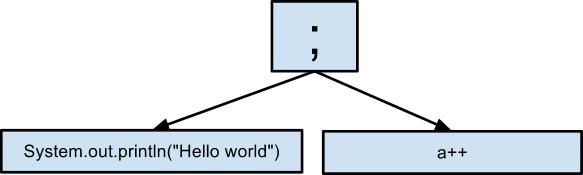
\includegraphics[width=0.8\textwidth]{seqTree}
	\caption{Последовательные операторы}
	\label{fig:seqImage}
\end{figure}

\begin{figure}[h!]
	\centering
	% \inputminted{c}{codes/seqCode1.java}
	\lstinputlisting[language=Java]{codes/seqCode1.java}
	\caption{Последовательные операторы в строчку}
	\label{fig:seqCode1}
\end{figure}

\begin{figure}[h!]
	\centering
	% \inputminted{c}{codes/seqCode2.java}
	\lstinputlisting[language=Java]{codes/seqCode2.java}
	\caption{Последовательные операторы в несколько строк}
	\label{fig:seqCode2}
\end{figure}


Рассмотрим другой пример.
Пусть нам нужно текстовое представление синтаксического дерева конструкции
“\lstinline{if}”, и заданы шаблоны c рис.~\ref{fig:ifTemplate2} и
\ref{fig:ifTemplate1}. При этом вариант, изображенный на
рис.~\ref{fig:ifTemplate2} выбирается только в случае, если условие и
ветки могут быть напечатаны в одну строчку.

\begin{figure}[h!]
	\subfloat[]{
		\lstinputlisting[language=Haskell]{codes/ifTemplate2.hs}
		\label{fig:ifTemplate2}	
	}
	\quad
	\subfloat[]{
		\lstinputlisting[language=Haskell]{codes/ifTemplate1.hs}
		\label{fig:ifTemplate1}	
	}
	\caption{Представления для конструкции “\lstinline{if}”}
\end{figure}


Тогда для деревьев, представленных на рис.
\ref{fig:ifImage1} и \ref{fig:ifImage2}, будут напечатаны коды с
рис. \ref{fig:ifCode1} и \ref{fig:ifCode2} соответственно.

\begin{figure}[h!]
	\subfloat[]{
		\centering
		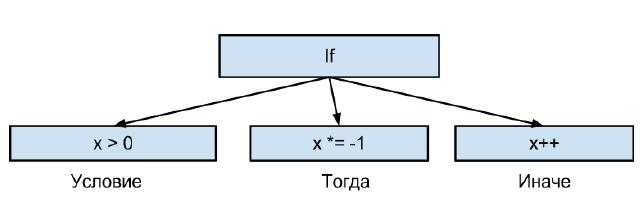
\includegraphics[width=0.6\textwidth]{if1}
		\label{fig:ifImage1}
	}
	\quad
	\subfloat[]{
		\centering
		% \inputminted{haskell}{codes/ifCode1.hs}
		\lstinputlisting[language=Haskell]{codes/ifCode1.hs}
		\label{fig:ifCode1}	
	}

	\caption{Использование представления с рис.~\ref{fig:ifTemplate2}}
\end{figure}

\begin{figure}[h!]
	\subfloat[]{
		\centering
		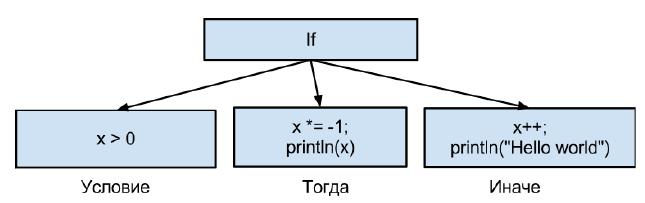
\includegraphics[width=0.6\textwidth]{if2}
		\label{fig:ifImage2}
	}
	\quad
	\subfloat[]{
		\centering
		% \inputminted{haskell}{codes/ifCode1.hs}
		\lstinputlisting[language=Haskell]{codes/ifCode2.hs}
		\label{fig:ifCode2}	
	}

	\caption{Использование представления с рис.~\ref{fig:ifTemplate1}}
\end{figure}

Существует несколько подходов к написанию принтеров.
Классическим способом задания принтеров в функциональных языках
программирования являются
принтер-комбинаторы~\cite{wadler, swierstra, swierstraChitil,
swierstra04, hughes, peytonJones, kiselyov, chitil, swiComb}.
Кроме того, существует работа, посвященная совместной разработке
принтера и синтаксического анализатора~\cite{rendelInvert}.
В \cite{jongeEveryOccasion, jongeReengine, brandBox} описаны методы
создания принтеров с помощью специализированных грамматик.

К сожалению, принтеры, создаваемые с помощью упомянутых подходов,
слабопараметризуемы и сложны. Чтобы избежать подобных проблем,
можно использовать шаблоны для описания представлений синтаксических
конструкций. Принципиальная возможность осуществления такого способа была
доказана в рамках предыдущей работы
автора. В \cite{myCoursePaper} был разработан
обобщенный принтер для учебного языка L, использующий расширяемый
синтаксический анализатор целевого языка для получения шаблонов.

Целью данной работы является разработка метода задания принтеров с помощью
образцов для языков программирования. 
Для апробирования метода было принято решение разработать принтер-плагин
языка Java для среды разработки IntelliJ IDEA\footnote{\cd{http://www.jetbrains.com/idea/}}.
В ходе разработки данного метода возникла необходимость улучшить существующую
принтер-комбинаторную библиотеку\cite{swierstra}. 

% Они вводят отношение \emph{частичного изоморфизма} на множествах абстрактных
% и конкретных синтаксических деревьев. Введение такого отношения позволяет
% совместно разрабатывать принтер и синтаксический анализатор. Кроме того,
% что таким образом уменьшается общий объем работы, подобный подход позволяет
% избежать несоответствия между принтером и анализатором.

% Вообще-то под \emph{комбинатором} понимается
% $\lambda$-терм без свободных переменных, но в нашем контексте о нем можно
% думать несколько проще --- как о функции высшего порядка,
% которая позволяет комбинировать сложный принтер из более простых.

\newpage
\section{Обзор}

\subsection{Принтер-комбинаторы}

Базовыми принтер-комбинаторными библиотеками являются библиотеки
Джона Хьюза\cite{hughes} и Филиппа Вадлера\cite{wadler}, которые
представляют собой функциональную реализацию алгоритма
Оппена\cite{oppen}.
Ограничимся рассмотрением библиотеки Вадлера, так как
библиотека Хьюза не отличается принципиально
в рамках данного рассуждения.

В библиотеке ключевым типом является документ.
Он представляет сущность, которая потом может
быть переведена в строковое представление алгоритмом принтера.
Основные конструкторы для составления документа:
\begin{itemize}
  \item атомарная строка, которая печатается как есть;
  \item \emph{разделитель};
  \item последовательная композиция двух документов;
  \item набор связанных документов.
\end{itemize}

Определяющей особенностью данного подхода является то, что все разделители
в рамках одного набора могут быть совместно заменены алгоритмом принтера
на пробельный символ или на перевод строки. Выбор для каждого набора разделителей
основывается на том, что вывод должен поместиться в заданную ширину,
используя минимальное число строк.

Основная проблема такого подхода заключается в его слабой выразительной силе.
Документы, построенные по синтаксическому дереву печатаемой программы,
обрабатываются слишком единообразно, что иногда приводит к нежелательному результату.
Пусть, к примеру, нужно напечатать программу на языке Python\footnote{Язык Python,
http://python.org}.
Между последовательными операторами, в случае их печати на одной строчке, необходимо
добавить дополнительный разделитель (``;''), иначе программа станет некорректной
(см. рис.~\ref{fig:seqEx}). Однако, описанные принтер-комбинаторы не предоставляют
возможности задать такое поведение.
Кроме того, с помощью таких принтер-комбинаторов невозможно выразить разные проектные СК,
так как они всегда печатают текст в одном стиле, который жестко зашит в их код.

\begin{figure}[h!]
	\centering
	\null\hfill
	\subfloat[Корректный код]{
		\centering
    \makebox[.4\textwidth] {
		  \lstinputlisting[language=Python]{codes/pythonCode.py}
    }
	}
	\null\hfill
	\subfloat[Некорректный код]{
		\centering
    \makebox[.4\textwidth] {
	  	\lstinputlisting[language=Python]{codes/pythonCodeBad.py}
    }
	}
	\hfill\null
	\caption{Пример работы принтер-комбинаторов для языка Python}
  \label{fig:seqEx}	
\end{figure}

Более подробный обзор библиотек Хьюза и Вадлера есть в предыдущей работе\cite{myCoursePaper}.

Большинство принтер-комбинаторных библиотек\cite{
swierstraChitil, swierstra04, peytonJones, kiselyov, chitil}
являются развитиями работ Хьюза и Вадлера. Так, в отличие от базовых, среди
них есть реализации с линейной сложностью обработки документа от его размера и
\emph{on-line} алгоритмы, которые не требуют просмотра всего документа
для начала печати его текстового представления. Но все они обладают тем же
интерфейсом, а значит в них также неразрешимы задачи, в которых требуется
задавать варианты текстовых представлений, которые отличаются не только
пробелами и переводами строк.

\subsection{Принтер-комбинаторы с выбором}

Существенно от описанных выше отличаются библиотеки, предоставляющие в своем
интерфейсе комбинатор \emph{выбора}, который позволяет задавать для одного поддерева
принципиально разные варианты раскладок.
Так в работах~\cite{jongeEveryOccasion, jongeReengine} используется оператор ``ALT'',
но алгоритм принтера устроен так, что среди двух альтернатив выбирается первая, если она
помещается в заданную ширину, и вторая иначе, что не дает оптимальный результат на выходе.

Оптимальные принтер-комбинаторы с выбором были впервые представлены в работе~\cite{swierstra}.
Их реализация является частью Utrecht Tools Library\footnote{
UTL, \cd{http://www.cs.uu.nl/wiki/HUT/WebHome}} (практическая реализация несколько изменена по
отношению к той, что описана в статье, но отличие несущественно).
В данном подходе текст строится из блоков прямоугольной формы с возможно неполной последней
строчкой (см. рис. \ref{fig:basicFormat}). В реализации на Haskell блоки представляются
структурой \lstinline[language = Haskell]{Format}:
\begin{lstlisting}
    data Format = Elem { height        :: Int
                       , lastLineWidth :: Int
                       , width         :: Int
                       , txtstr        :: Int -> String -> String
                       }
\end{lstlisting}

Первые три поля структуры определяют геометрические размеры блока, а последнее --- функция,
которая используется для преобразования блока в текст. Здесь используется функция, а не
просто строчка, чтобы можно было преобразовывать вложенные блоки за линейное время. Первый
аргумент \lstinline[language = Haskell]{txtstr} задает сдвиг блока.

\begin{figure}
  \centering
  \subfloat[Блок Format]{
    \raisebox{5mm}{
      \centering
      \vspace{0pt}
      \tikz[scale = 2.0]{
        \draw (0,0) -- (1,0) -- (1,0.2) -- (2,0.2) -- (2,1) -- (0, 1) -- cycle;
      }
    }
    \label{fig:basicFormat}
  }
  ~
  \subfloat[Горизонтальная композиция]{
    \centering
    \tikz[scale = 2.0]{
       \draw (0,0) -- (1,0) -- (1,0.2) -- (2,0.2) -- (2,1) -- (0, 1) -- cycle;
       \draw (1.1,-0.9) -- (2.1,-0.9) -- (2.1,-0.7) -- (3.1,-0.7) -- (3.1,0.1) -- (1.1,0.1) -- cycle;
     }
     \label{fig:beside}
  }
  %\hfill
  ~
  \subfloat[Вертикальная композиция]{
    \makebox[.28\textwidth] {
    \centering
    \tikz[scale = 2.0]{
       \draw (0,0) -- (1,0) -- (1,0.2) -- (2,0.2) -- (2,1) -- (0, 1) -- cycle;
       \draw (0,-1.1) -- (1,-1.1) -- (1,-0.9) -- (2,-0.9) -- (2,-0.1) -- (0,-0.1) -- cycle;
    }
    \label{fig:above}
    }
  }
  \caption{Примитивы структуры Format}
  \label{fig:basicConcat}
\end{figure}

Для работы с \lstinline[language = Haskell]{Format} используется следующие 4 примитива:
\begin{lstlisting}
    s2fmt     :: String -> Format
    indentFmt :: Int -> Format -> Format
    aboveFmt  :: Format -> Format -> Format
    besideFmt :: Format -> Format -> Format
\end{lstlisting}

Функция \lstinline[language = Haskell]{s2fmt} создает \lstinline[language = Haskell]{Format},
состоящий из одной строчки; \lstinline[language = Haskell]{indentFmt} по блоку создает новый,
сдвинутый на заданное число позиций. Действие примитивов композиции
\lstinline[language = Haskell]{besideFmt} и \lstinline[language = Haskell]{aboveFmt}
показано на рисунках \ref{fig:beside} и \ref{fig:above} соответственно.

Также, как и в библиотеках без комбинатора выбора, в данной работе используется понятие
\emph{документа}. Здесь документ можно рассматривать как множество возможных раскладок
(набор \lstinline[language = Haskell]{Format}-элементов). Документы описываются типом
\lstinline[language = Haskell]{Doc}, который на этапе построения представляет собой
дерево применений комбинаторов (приведены ниже), а на этапе обработки алгоритмом
принтера ему в соответствие ставится итоговое множество вариантов.

Документ конструируется с помощью следующих комбинаторов, которые симметричны
примитивам построения блоков \lstinline[language = Haskell]{Format}:
\begin{lstlisting}
    text   :: String -> Doc
    indent :: Int -> Doc -> Doc
    beside :: Doc -> Doc -> Doc
    above  :: Doc -> Doc -> Doc
\end{lstlisting}

В дополнение появляется пятый комбинатор для документов:
\begin{lstlisting}
    choice :: Doc -> Doc -> Doc
\end{lstlisting}

Этот комбинатор и является тем самым комбинатором выбора. Он представляет
\emph{объединение} множеств раскладок документов, которые были переданы как
аргументы комбинатора. Заметим, что только этот комбинатор может произвести
документ с несколькими раскладками из одновариантных аргументов.

Оригинальная реализация сильно завязана на ленивые вычисления. В \cite{swierstra}
множество вариантов, соответствующее экземпляру \lstinline[language = Haskell]{Doc},
представляется ленивым списком всех возможных раскладок, удовлетворяющих ограничению
на максимальную ширину. Этот список отсортирован в порядке \emph{``ухудшения''}
раскладок, то есть в голове списка лежит \emph{``лучшая''}, в терминах оптимальности,
раскладка из возможных при заданной ширине. В случае ``beside'' и ``above'' композиций
документов полная (без учета ленивости) сложность вычисления списка нового документа
составляет $O(n \times m)$, где $n$ и $m$ --- размеры соотвествующих списков,
соединяемых документов. Также размер нового списка является $O(n \times m)$.

Выбор лучшего представления для самого верхнеуровнего документа происходит
просто --- нужно из соотвествующего списка взять первый элемент. Поэтому
на первый взгляд кажется, что общее число вычислений существенно уменьшается,
благодаря ленивым вычислениям. Но это не так из-за реализации обработки документа,
построенного с помощью комбинатора \lstinline[language = Haskell]{beside}, которая
форсирует полное вычисление дочерних списков. Так, обработка документа в
\cite{swierstra} имеет в худшем случае экспоненциальную сложность от числа
комбинаторов, использованных при его построении.
В \cite{swiComb} приведены оптимизации к этому подходу, но они
не улучшают асимптотику решения.

\newpage
\subsection{Средства форматирования кода в IDE}

Интегрированные среды разработки программного обеспечения
(IDE) предоставляют средства
для форматирования программного кода. Рассмотрим их на примере двух Java IDE ---
IntelliJ IDEA и Eclipse\footnote{Eclipse IDE, \cd{http://eclipse.org}}.
Для задания требуемого СК используется широкий набор настроек \textbf{форматтера},
подпрограммы IDE, отвечающей за форматирование исходных текстов.
Примерами таких настроек являются:
\begin{itemize}
  \item помещать ли фигурную скобку на той же строке, что и
    предыдущее выражение;
  \item форматирование списков --- всегда на одной строчке, переводить строчку после
    каждого элемента или печатать на одной строке,
    пока строчка меньше заданной рекомендуемой ширины;
  \item и т.д.
\end{itemize}
На рисунках~\ref{fig:ideaFormatter} и~\ref{fig:eclipseFormatter} приведены диалоги задания
параметров форматирования в IntelliJ IDEA и Eclipse соответственно.

\begin{figure}[p]
	\centering
	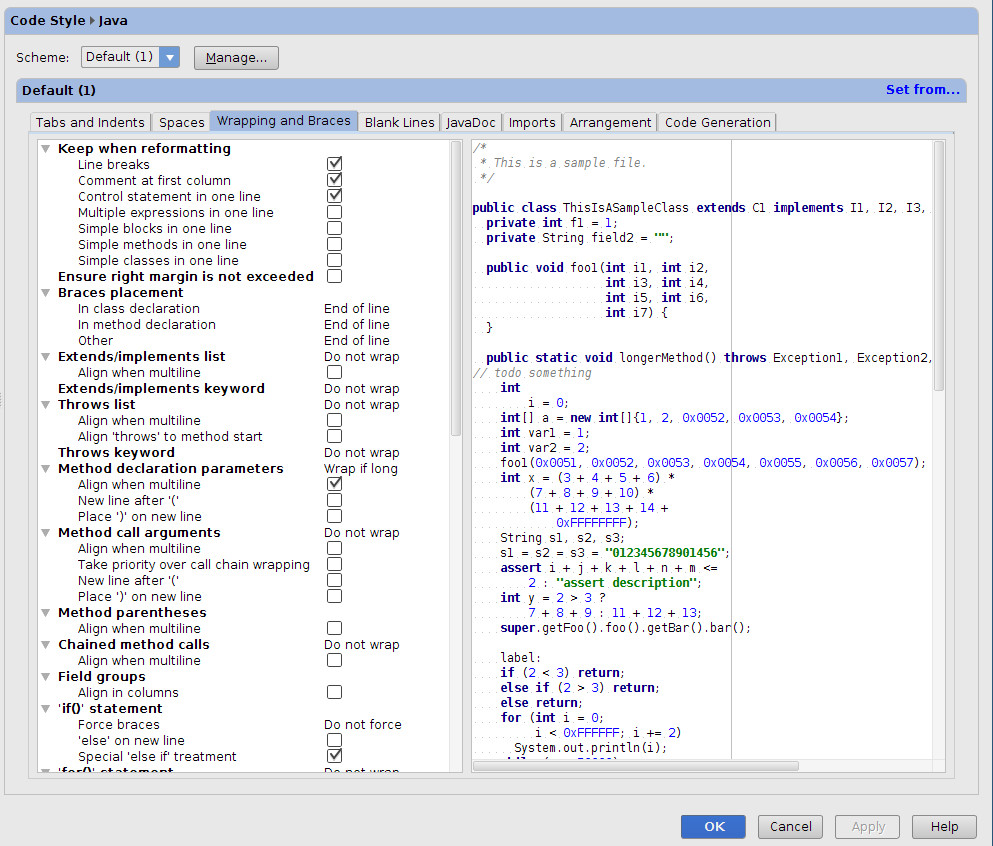
\includegraphics[width=\textwidth]{ideaFormatter}
	\caption{Окно настройки форматтера IntelliJ IDEA}
	\label{fig:ideaFormatter}
\end{figure}

\begin{figure}[p]
	\centering
	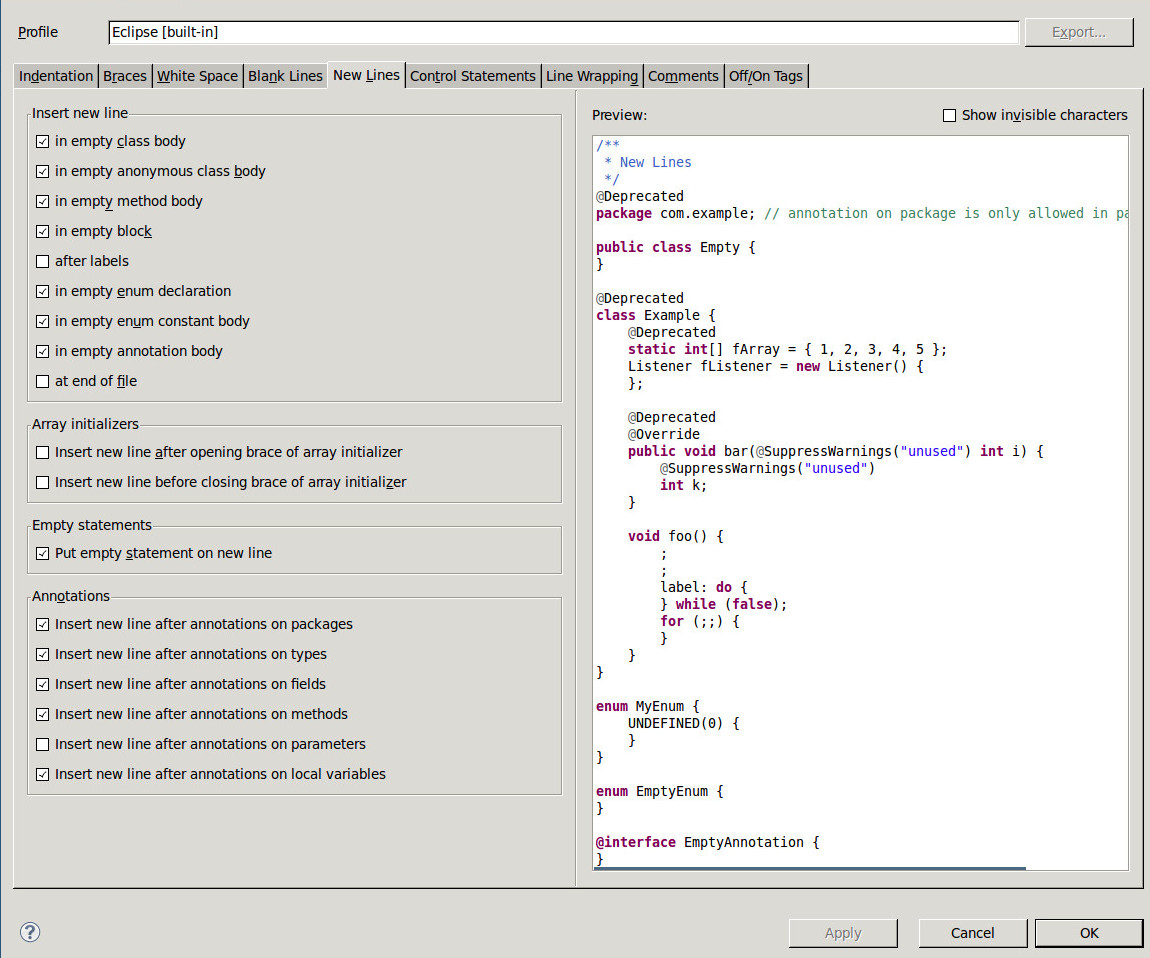
\includegraphics[width=\textwidth]{eclipseFormatter}
	\caption{Окно настройки форматтера Eclipse}
	\label{fig:eclipseFormatter}
\end{figure}

У встроенных форматтеров есть следующие особенности.
Во-первых, это невозможность выразить
оригинальный СК, так как настройки форматтеров, несмотря на их большое
количество,
дают ограниченную вариативность для текстовых представлений форматируемых
программ. В целом,
стили форматирования, которые можно задать с помощью данных настроек,
ограничиваются парой стандартных.
Во-вторых, в случае если надо
придерживаться СК уже существующего проекта, то по коду этого проекта необходимо
вручную задать все настройки форматтера.
Причем наборы настроек в разных IDE не совпадают, что увеличивает сложность
поддержки единого СК, если разработчики используют отличные от друг друга IDE.
Для решения данной проблемы существуют плагины, позволяющие использовать
внешние фоматтеры\footnote{Плагин к IntelliJ IDEA, позволяющий использовать
встроенный форматтер Eclipse, \cd{http://plugins.jetbrains.com/plugin/6546}}.
Кроме того, есть средства, позволяющие экспортировать настройки форматтера в
XML-файл, для их использования в другой
IDE\footnote{Импортирование настроек форматтера из Eclipse в IntelliJ IDEA,
\cd{http://blog.jetbrains.com/idea/2014/01/intellij-idea-13-importing-code-formatter-settings-from-eclipse/}}.

Важным достоинством описанных принтеров является малое время работы.
Это достигается в том числе и за счет того, что часто форматируется не весь
файл, а только его часть~\cite{eclipse},
и из-за детерминированности самого алгоритма, которая следует из специфики
настроек форматтера.
Однако форматирование целого большого проекта занимает существенное время.
Например, форматирование кода IntelliJ IDEA Community Edition занимает более часа
у встроенного в IDEA форматтера.

\newpage
\subsection{BURS}

Bottom-Up Rewrite System (BURS)\cite{burs} --- это метод динамического
программирования на деревьях, изначально появившийся в контексте задачи выбора
набора инструкций для генерации машинного кода. Основой BURS является
регулярная древесная грамматика\cite{tata} со стоимостью применения подстановки,
то есть грамматика со следующим набором правил: 

$$
\begin{array}{rcll}
  N &:& \alpha& [c]\\
  N &:& \alpha\; (K_1,\dots,K_n)& [c]
\end{array}
$$

Здесь $N, K_i$ это нетерминалы, $\alpha$ --- терминал,
$c$ --- функция цены, описанная для каждого правила.
Как и для обычной линейной грамматики, вводится стартовый
нетерминал S. Считается, что терминальное дерево выводится в
данной грамматике, если его можно получить с помощью правил
подстановки из одноузлового дерева $S$.
Каждая подстановка заменяет нетерминал $N$, находящийся в листе дерева, на дерево 
$\alpha\;(K_1,\dots,K_n)$, если в грамматике есть правило
$N:\alpha\;(K_1,\dots,K_n)$. 
Для каждой подстановки вычисляется стоимость ее применения с помощью
функции цены ($c$).
Аргументами функции могут служить терминальная метка ($\alpha$) и стоимости
вывода поддеревьев.
Задачей, которую решает BURS, является поиск вывода наименьшей стоимости
для заданного дерева по заданной грамматике.
Такой вывод может быть найден двухпроходным алгоритмом.

Первый проход (\emph{пометка}) обрабатывает дерево снизу вверх и вычисляет
для каждого узла набор троек $(K,\;R,\;c)$, где $K$ --- нетерминал, из которого может быть
выведено поддерево с корнем в обрабатываемом узле,
$R$ --- первое правило, которое используется для вывода минимальной стоимости из $K$,
$c$ --- стоимость такого вывода.
Процесс пометки происходит следующим образом:

\begin{itemize}
\item для листовой вершины, помеченной терминалом $\alpha$, в множество троек
этого вершины добавляется $(K,\;R,\;c\:(\alpha))$ для каждого правила $R=K:\;\alpha\;[c]$;
\item для промежуточной вершины, помеченной терминалом $\alpha$,
с непосредственными поддеревьями $v_1,\dots,v_n$
в множество добавляется тройка $(K,\;R,\;c\:(\alpha,c_1,\dots,c_n))$ для каждого правила
$R=K:\;\alpha\;(K_1,\dots,K_n)\;[c]$, где $(K_i,\;R_i,\;c_i)$ входит в множество троек для
$v_i$; если есть несколько правил вывода из нетерминала $K$, то выбирается правило,
минимизирующее стоимость вывода.
\end{itemize}

Второй проход (\emph{свертка}) просматривает дерево сверху вниз, используя сделанные пометки.
Первое правило из минимального вывода определяется тройкой $(S,\;R,\;c)$ для корневого узла
(если такой тройки нет, то вывод из $S$ невозможен).
Это правило однозначно определяет нетерминалы $K_i$ для каждого непосредственного поддерева
и процесс повторяется.

Для пометки дерева потенциально необходимо каждое правило грамматики применить к каждому узлу.
При фиксированной грамматике алгоритмическая сложность первого прохода --- $O\:(|R|)$,
где $|R|$ --- количество правил
(размер множества троек для каждого узла ограничен числом нетерминалов, которое не больше,
чем количество правил). Свертка также имеет линейную сложность.


\subsection{Язык программирования Kotlin}

Язык Kotlin это функциональный, объектно-ориентированный язык,
разрабатываемый в компании JetBrains.
Kotlin был выбран для реализации принтер-плагина к IDEA по нескольким причинам. 
Во-первых, Kotlin обладает хорошей интеграцией с Java, что позволяет
использовать его без проблем с IDEA API. 
Во-вторых, функции в Kotlin являются объектами первого рода, что позволяет
легко реализовывать комбинаторные библиотеки на нем.
На данный момент Kotlin находится в стадии разработки, поэтому
периодически возникают
проблемы с тем, что исходные коды перестают быть совместимыми с новыми
версиями языка,
но обычно требуется внести небольшой набор исправлений для
восстановления работоспособности.

\newpage
\section{Реализация}

\subsection{Сведение Pretty-Printing к BURS}
Для снижения алгоритмической сложности задачи поиска
оптимального представления документа, заданного комбинаторами из \cite{swierstra},
можно произвести сведение к BURS.
Сведение основано на следующих наблюдениях. Пусть $w$ есть максимальная допустимая
ширина вывода. Поскольку каждая возникающая раскладка представляется блоком
\lstinline[language=Haskell]{Format}, для поиска оптимального представления можно рассматривать
все промежуточные раскладки
как тройки $(n, k, h)$, где $n \le w$ --- это общая ширина раскладки, $k \le n$ ---
ширина ее последней строчки, $h$ --- ее высота. Тогда очевидно, что при $h_1 \le h_2$
между $(n, k, h_1)$ и $(n, k, h_2)$ первая тройка предпочтительней на любом этапе вычислений.
Таким образом для каждого узла не может быть более $w^2$ существенных представлений\footnote{
На самом деле, из-за ограничения $k \le n$ максимальное число раскладок не $w^2$, a
$\frac{w^2 + w}{2}$, но это несущественно.}.

Документ, для которого мы ищем раскладку, можно рассматривать как дерево, построенное из примитивов
\lstinline[language=Haskell]{text},
\lstinline[language=Haskell]{indent},
\lstinline[language=Haskell]{beside},
\lstinline[language=Haskell]{above} и \lstinline[language=Haskell]{choice}. Тогда задачу
раскладки документа можно решать независимо для поддеревьев, а потом объединять решения
при учете, что для каждого поддерева
и каждой пары $(n, k), k \le n \le w$ запоминается минимальная $h$ такая, что для поддерева существует
текстовое представление с размерами $(n, k, h)$. Тогда, совершив обход дерева снизу вверх, мы сможем
вычислить оптимальное представление для всего дерева. Полезно заметить,
что оптимальное представление дерева не всегда получается из оптимальных представлений его
поддеревьев, поскольку при использовании поддеревьев возникают дополнительные
ограничения на ширину раскладок этих поддеревьев.

Приведенные наблюдения можно формализовать в виде BURS-задачи.
Для заданной ширины вывода $w$ введем набор нетерминалов
$T_n^k$, для всех $k \le n \le w$. Определим BURS-грамматику так, чтобы цена вывода $h$ нетерминала
$T_n^k$ для документа соответствовала его раскладке с параметрами $(n, k, h)$.
Для такой BURS-грамматики этап разметки посчитает все существенные раскладки, а этап свертки
вернет оптимальную. Определим правила переписывания для этой грамматики:
\begin{enumerate}
\item Для терминального узла $[\mbox{\lstinline{text s}}]$\footnote{
  Квадратные скобки используются для обозначения терминалов, состоящих из одного
  или нескольких символов.}
  существует два варианта:
  \begin{itemize}
     \item Если $|s|\le w$ (где $|s|$ --- это длина строки $s$), то вводится единственное правило
           $T^{|s|}_{|s|}: [\mbox{\lstinline{text s}}]$ со стоимостью $1$;
           
           для всех остальных
           $k, n\ne |s|$ используется $T^k_n:[\mbox{\lstinline{text s}}]$ со стоимостью $\infty$;
     \item Если $|s| > w$, то используется $T^k_n:[\mbox{\lstinline{text s}}]$ со стоимостью\
       $\infty$ для всех $k, n$.
  \end{itemize}
  Действительно, раскладка документа, состоящего из строчки длины $|s|$, может быть только размеров
  $(|s|, |s|, 1)$. Все остальные размеры недоступны, поэтому имеют стоимости $\infty$.

\item Для узла $[\mbox{\lstinline{indent m}}]$ введем два набора правил:
  \begin{enumerate}
     \item $T^{k+m}_{n+m}:[\mbox{\lstinline{indent m}}]\:(T^k_n)$ со стоимостью,
       равной стоимости раскладки поддерева $m$ в $T_n^k$, для всех $n$ 
     и $k$ таких, что $n+m\le w$ и $k\le n$;
     \item $T^k_n:[\mbox{\lstinline{indent m}}]\:(T^i_j)$ со стоимостью $\infty$ в противном случае.
  \end{enumerate}
  Понятно, что сдвиг раскладки с параметрами $n$, $k$ и $h$ на $m$ позиций вправо
  создает раскладку с параметрами $n+m$, $k+m$, $h$. Такая раскладка допустима, если
  $n+m\le w$ и $k+m\le w$.

\item Для узла $[\mbox{\lstinline{above}}]$ вводим правило $T^{k_2}_{\max(n_1, n_2)}:[\mbox{\lstinline{above}}]\:(T^{k_1}_{n_1},\;T^{k_2}_{n_2})$ 
со стоимостью, равной сумме стоимостей вывода поддеревьев,
для всех $k_1\le n_1\le w$ и $k_2 \le n_2 \le w$.

Действительно, при вертикальном соединении раскладок с параметрами
$n_1$, $k_1$, $h_1$ и $n_2$, $k_2$, $h_2$ мы получаем раскладку с размерами
$\max\:(n_1,n_2)$, $k_2$, $h_1+h_2$. Вертикальная композиция допустимых раскладок всегда допустима.

\item Для узла $[\mbox{\lstinline{beside}}]$ вводим правило
  $T^{k_1+k_2}_{\max\:(n_1,\:k_1+n_2)}:[\mbox{\lstinline{beside}}]\:(T^{k_1}_{n_1},\:T^{k_2}_{n_2})$
  для каждой комбинации $n_1, n_2, k_1, k_2$ такой, что $k_1+k_2\le\max\:(n_1,\:k_1+n_2)\le w$.
  Стоимость такого вывода равна сумме стоимостей вывода поддеревьев минус 1.
  Это может быть легко проверено из геометрических соображений.

\item Для узла $[\mbox{\lstinline{choice}}]$ вводим правило
  $T^k_n:[\mbox{\lstinline{choice}}]\:(T^k_n,\:T^k_n)$ для всех $k\le n\le w$.

  Цена есть минимум среди цен вывода для поддеревьев. Понятно, что среди двух раскладок
  с одинаковыми ширинами выбирается та, что имеет меньшую высоту.
\end{enumerate}

Для завершения описания грамматики необходимо ввести правило для стартового нетерминала $S$.
Можно добавить правило $S : r$ с тождественной функцией цены для любого $r$, или ввести
цепное правило $S: T_n^k$ с такой же функцией для всех нетерминалов $T_n^k$
(такое правило требует несущественного расширения определения BURS).

Число нетерминалов в определенной выше грамматике есть $O(w^2)$.
Однако, число правил есть $O(w^4)$, так
как в дереве есть узлы со степенью 2. Так, приведенная BURS реализация оптимального принтера
работает за линейное время от числа узлов в дереве документа для фиксированной ширины вывода, при
этом сложность от ширины вывода есть $O(w^4)$. Понятно, что данное сведение может быть выполнено и
для других примитивов построения дерева, которые могут иметь большую степень, но ценой
экспоненциального роста сложности по $w$.
\label{txt:bursReduction}


\newpage
\subsection{Библиотека принтер-комбинаторов на Haskell}

В рамках данной работы удалось реализовать
принтер-комбинаторную библиотеку (см. приложение~\ref{app:1}) с тем же набором комбинаторов,
что и в~\cite{swierstra},
которая линейна относительно входного документа и полиномиальна
относительно максимальной ширины вывода, за счет описанного выше сведения задачи к BURS.
Данная реализация использует низкоуровневые типы и функции из оригинальной
библиотеки~\cite{swierstra}, в то время как высокоуровневые типы и комбинаторы переопределены.

В реализации нет непосредственного использования BURS: в явном виде не задается BURS-грамматика,
нет набора нетерминалов и стандартного алгоритма обработки.
Вместо этого для каждого узла документа вычисляется ассоциативный массив, который
ставит в соответствие паре $(n, k)$ лучший (минимальный по числу строк) Format с параметрами
ширин $n$ и $k$. Так, в ассоциативном массиве записаны пары $((n, k), f)$, где $f$ --- это
блок Format, соответствующий оптимальному представлению с ширинами $(n, k)$. Значение
высоты $f$ есть минимальная стоимость вывода нетерминала $T^k_n$ для данного узла.
Заметим, что поскольку $f$ является конечным результатом для $T^k_n$, а не просто
последним правилом, которое нужно применить для построения ответа, то отменяется
необходимость применения в дальнейшем алгоритма свертки.
В конце, для корня дерева, представляющего документ, выбирается элемент минимальной стоимости из
ассоциативного массива.

Наибольший интерес в рамках данного исследования представляет поведение библиотеки
в худшем случае.
Реализация была апробирована для бинарных деревьев.
Функция генерации деревьев приведена на рисунке~\ref{fig:treeToDocMy}.
Здесь используются операторы
\lstinline[language= Haskell]{(>|<)},
\lstinline[language= Haskell]{(>-<)},
\lstinline[language= Haskell]{(>//<)}, которые являются инфиксными синоминами для
комбинаторов
\lstinline[language= Haskell]{beside},
\lstinline[language= Haskell]{above} и
\lstinline[language= Haskell]{choice} соответственно.

\begin{figure}[h!]
  \lstinputlisting[language = Haskell]{codes/AltPrettyTest.hs}
  \caption{Функция генерации деревьев для тестов производительности}
  \label{fig:treeToDocMy}
\end{figure}

Результаты времени исполнения для сравнения авторской реализации с оригинальной библиотекой
приведены в таблице~\ref{tbl:time}.
Из приведенных данных видно, что, начиная с некоторой комбинации ширины вывода и размера документа,
библиотека~\cite{swierstra} не может вычислить раскладку документа.
Значения, записанные подобно \mbox{``-($>$ 59)''}, обозначают,
что после указанного времени процесс аварийно завершился с переполнением стека.

Авторская реализация часто не показывает линейное поведение, как это ожидается при фактическом
учетверении числа узлов в документе от строчки к строчке. Дополнительные эксперименты показали
связь данного поведения с разреженностью ассоциативного массива для больших ширин.
Другими словами, для маленьких деревьев число значений в соответствующем ассоциативном массиве
сильно меньше верхней границы. С ростом размера дерева число записей растет быстрее чем
с линейной скоростью, пока не будут достигнуты значения, близкие к верхней границе.

Кроме того, особенностью описанной реализации является то, что она не использует 
ленивые вычисления для ускорения построения оптимального текстового представления для
поданного на вход документа, а, наоборот,
форсирует большинство вычислений, что делает ее легко портируемой на языки
без встроенной ленивости.

Полные исходные коды библиотеки вместе с тестами можно найти на

\cd{http://github.com/anlun/polynomialPPCombinators}.

\begin{table}[h!]
	\centering
	\subfloat[Ширина вывода 25] {
		\centering
		\begin{tabular}{c c c}
		Число узлов & Оригинальная & Авторская \\ 
		\hline
		10921 & 0.07 & 0.18 \\
		43689 & 1.28 & 0.73 \\
		174761 & 6.47 & 2.86 \\
		699049 & 18.46 & 11.58 \\
		2796201 & 46.54 & 47.52 \\
		11184809 & 98.85 & 187.90 
		\end{tabular}
	}
	\quad
	\subfloat[Ширина вывода 50] {
		\centering
		\begin{tabular}{c c c}
		Число узлов & Оригинальная & Авторская \\ 
		\hline
		10921 & 0.12 & 0.69 \\
		43689 & 287.55 & 4.03 \\
		174761 & - (\textgreater 294) & 17.93 \\
		699049 & - (\textgreater 284) & 71.70 \\
                \phantom{ }&&\\
                \phantom{ }&&
		\end{tabular}
	}

	\quad
	\subfloat[Ширина вывода 100] {
		\centering
		\begin{tabular}{c c c}
		Число узлов & Оригинальная & Авторская \\
		\hline
		10921 & 0.06 & 0.97 \\
		43689 & 97.79 & 14.92 \\
		174761 & - (\textgreater 179) & 88.71 
		\end{tabular}	
	}
	\quad
	\subfloat[Ширина вывода 150] {
		\centering
		\begin{tabular}{c c c}
		Число узлов & Оригинальная & Авторская \\ 
		\hline
		10921 & 0.06 & 1.01 \\
		43689 & 38.99 & 20.75 \\
		174761 & - (\textgreater 59) & 204.51 
		\end{tabular}	
	}

	\caption{Время вычисления раскладки (в секундах)}
	\label{tbl:time}
\end{table}



\newpage
\subsection{Библиотека принтер-комбинаторов на Kotlin}

Для дальнейшего использования в принтер-плагине, авторская библиотека комбинаторов была
переписана на язык Kotlin. Данная реализация расширяет набор комбинаторов и использует
дополнительные техники, которые важны при практическом применении библиотеки.

\subsubsection{Мемоизация вычислений для поддеревьев}

В реальных принтерах документы, состоящие из комбинаторов
\lstinline[language=Haskell]{text},
\lstinline[language=Haskell]{indent},
\lstinline[language=Haskell]{beside},
\lstinline[language=Haskell]{above} и \lstinline[language=Haskell]{choice}, чаще всего
представляют собой не дерево, а \textit{дэг} (DAG, Direct Acyclic Graph). Поэтому при наивной
реализации можно получить экспоненциальную сложность от размеров документа,
поскольку соответствующее дерево будет иметь экспоненциальный размер от размера дэга.
Чтобы избежать этой проблемы достаточно завести ассоциативный массив,
который будет хранить посчитанный набор раскладок по конкретному поддереву.
Опять же при наивной реализации данной оптимизации,
алгоритм вычисления раскладки становится квадратичным от размера дэга,
так как вычисление хэша, используемого ассоциативным массивом, для дерева занимает
линейное время. Чтобы преодолеть и эту сложность, в дереве хранится вычисленный хэш.

\subsubsection{Комбинатор Fill}

Для реализации принтера, использующего шаблоны, необходимо добавить
дополнительный принтер-комбинатор в библиотеку --- комбинатор Fill.

\begin{figure}[h!]
  \centering
	\subfloat[]{
		\centering
    \tikz[scale = 2.5]{
       \draw (0,0) -- (1,0) -- (1,0.2) -- (2,0.2) -- (2,1) --
          (0, 1) -- cycle;
       \draw (0,-0.1) -- (0,-1.1) -- (1.1,-1.1) -- (1.1,-0.9) --
          (2.3,-0.9) -- (2.3, 0.1) -- (1.1,0.1) -- (1.1,-0.1) -- cycle;
    }
		\label{fig:fill1}
	}
	\quad
  \subfloat[][fc --- константа сдвига]{
		\centering
    \tikz[scale = 2.5]{
          \draw (0,0) -- (1,0) -- (1,0.2) -- (2,0.2) -- (2,1)
            -- (0, 1) -- cycle;
          \draw (0.3,-0.1) -- (0.3,-1.1) -- (1.1,-1.1) -- (1.1,-0.9)
            -- (2.3,-0.9) -- (2.3, 0.1) -- (1.1,0.1) -- (1.1,-0.1) -- cycle;
          \draw[<->] (0,-0.6) -- (0.3,-0.6);
          \draw (0.15,-0.4) node [fill=white] {\tiny fc};
          \draw[dashed] (0,0) -- (0,-1.1);
       }
		\label{fig:fill2}
	}
	\caption{Оператор Fill}
\end{figure}

В качестве примера, показывающего необходимость такого комбинатора, рассмотрим
печать метода из языка Java. Пусть нам нужно получить на выходе следующий программный
код:

\lstinputlisting[language = Java]{codes/codeBlockEx.java}

По описанному раннее подходу, для построения общей раскладки необходимо иметь представления
поддеревьев. В частности, представление тела метода:

\lstinputlisting[language = Java]{codes/justBlockEx.java}

Тогда для реализации необходимого соединения, представленного ниже, необходим комбинатор Fill:

\lstinputlisting[language = Java]{codes/codeBlockTemplateEx.java}

К сожалению, введение нового комбинатора накладывает дополнительные ограничения на
факторизацию. Это связано с тем, что теперь по парам $(n, k)$, где $n$ --- общая ширина,
а $k$ --- ширина последней строчки, нельзя однозначным образом выдать соответствующую
пару для раскладки соединения двух блоков. Так, при применении Fill комбинатора
важной становиться и ширина первой строчки нижнего блока, поскольку сумма ее и ширины
последней строчки верхнего блока могут дать максимум общей ширины. Таким образом,
у нетерминалов из BURS-сведения появляется дополнительный индекс, а их число
увеличивается с $w^2$ до $w^3$. Аналогично, количество правил перехода возрастает
с $O(w^4)$ до $O(w^6)$.

\subsubsection{Дополнительная фильтрация вариантов}

Для того, чтобы избежать экспоненциальной сложности вычисления оптимальной
раскладки документа, мы ввели факторизацию по размерам (ширинам) текстового
представления.
Количество раскладок для каждого поддерева теперь ограничено, но, к сожалению,
слишком большой константой --- $w^3$ ($w^2$ для набора комбинаторов без
Fill), а сложность вычисления узлов Beside, Above, Fill --- $O(w^6)$
($O(w^4)$ без комбинатора Fill). Факторизация была основана на том факте, что
среди раскладок с одинаковыми ширинами в любом дальнейшем использовании
к лучшему результату приводит вариант с меньшей высотой.
Для дополнительной фильтрации множества
вариантов воспользуемся рассуждением, что если раскладка $A$ обладает и
меньшими ширинами, и меньшей высотой, чем раскладка $B$, то, аналогично
предыдущей факторизации,
достаточно оставить только ее во множестве вариантов.

Таким образом мы ввели отношение частичного порядка на раскладках, а
описанная фильтрация --- поиск минимумов на множестве представлений\cite{poset}.
Наивная реализация поиска имеет квадратичную сложность от размера множества,
таким образом асимптотика алгоритма не ухудшается из-за этих дополнительных
действий. К сожалению, данная оптимизация и не улучшает поведение
в худшем случае, так как
можно привести пример, когда все множество раскладок с допустимыми ширинами
будет состоять из несравнимых элементов, но на практике количество вариантов
существенно сокращается, что делает весь подход применимым на реальных данных.

\newpage
\subsection{Принтер-плагин Java для IntelliJ IDEA}

\subsubsection{Подход задания принтера с помощью шаблонов}
Работа принтера разбивается на два этапа: подготовка шаблонов и непосредственно
печать синтаксического дерева.

На подготовительном этапе строится набор шаблонов. Для большей
конкретики уточним понятие шаблона: в этой работе под \emph{шаблоном} мы будем
понимать данные, которые дают возможность получить раскладки для родительского
узла по представлениям дочерних поддеревьев.
Фактически в реализации это размеченное дерево разбора
некоторой синтаксической конструкции, в котором по каждой метке можно выяснить
ограничения на представление соответствующих поддеревьев и описание, каким
образом нужная раскладка поддерева должна быть вставлена в шаблон (с помощью
комбинатора Beside или Fill).

Для получения шаблонов алгоритм проходит по переданному пользователем репозиторию с
эталонным исходным кодом. По каждому узлу деревьев разбора файлов из репозитория
строится шаблон соответствующей синтаксической конструкции. Важной особенностью
является то, что для дальнейшей печати конструкций, имеющих плавающие число
поддеревьев, необходимо иметь отдельный шаблон для каждой комбинации поддеревьев.
Так, к примеру, для конструкции \lstinline[language = Java]{if} языка Java
необходимо иметь не менее двух шаблонов --- с веткой \lstinline[language = Java]{else}
и без нее. В данном случае такое требование не кажется слишком обременительным, но
если рассмотреть случай Java-класса, то ситуация несколько хуже --- у него может не
быть списка модификаторов доступа, суперкласса и реализуемых интерфейсов.
Это серьезное ограничение, но его невозможно обойти в рамках данного подхода,
поскольку единственной информацией о представлении конструкций должны быть
полученные шаблоны.

Вычисление текстового представления переданного на вход синтаксического
дерева происходит путем восходящего переписывания. Для каждого узла строится множество
возможных раскладок (набор структур Format) по тем же правилам факторизации, чтобы были
применены для комбинаторной библиотеки. В дальнейшем представления поддеревьев
используются для подстановки в шаблоны родительского узла, что на выходе дает
набор раскладок для него. Шаблоны в данном контексте можно рассматривать как
BURS-правила. Однако, несмотря на то, что число детей у родительского узла может
быть велико (в случае некоторых конструкций языка Java более 5),
это не приводит к экспоненциальному росту сложности по ширине вывода, которые
следуют из рассуждений раздела \ref{txt:bursReduction}. Так, в общем случае применения
BURS-правила сложность вычисления должна составлять $O(w^{3 \times n})$, где $w$ ---
ширина вывода, а $n$ --- число дочерних поддеревьев обрабатываемого узла. Но
особенности подстановки раскладок в шаблон позволяют реализовать ее
за $O(n \times w^{6})$ для любого $n \geq 2$ ($O(w^{3})$ для $n = 1$).
Дополнительная техника позволяет снизить сложность подстановки в многострочный шаблон
до $O(n \times w^{4})$.

Таким образом, сложность вычисления сушественных раскладок для узла дерева
составляет $O(t \times n \times w^{6})$, где $t$ --- общее число шаблонов,
а в целом поиск оптимального представления всего синтаксического дерева, переданного
на форматирование, занимает $O(m \times t \times n \times w^{6})$, где $m$
--- количество узлов в дереве.


Стоит заметить, что с инженерной точки зрения для решения отдельно стоящей задачи
форматирования по образцу кода на Java в IntelliJ IDEA лучше подходит
получение настроек для существующего форматтера с помощью известных техник обучения.
Подобный подход используется в работе \cite{learning}.
Но описанный в данной работе метод позволяет выразить представления, которые не
предусмотрены встроенным форматтером, кроме того потенциально предоставляет
возможность проще создавать принтеры для новых языков. 

\subsubsection{Практические особенности получения и использования шаблонов}

Поскольку каждый узел дерева разбора из эталонного репозитория порождает
шаблон, то частой ситуацией является присутствие шаблонов, которые функционально
неотличимы. Их наличие ухудшает время работы принтера, так как повторяются
аналогичные переходы от представлений поддеревьев печатаемого узла, приводящие
к одному и тому же результату. Чтобы избежать данной проблемы достаточно ввести
факторизацию по функциональному поведению на множестве шаблонов. На практике это
было реализовано в виде факторизации по текстовому представлению шаблона,
в котором на месте меток записана информация об ограничении на раскладки
соответствующих поддеревьев.

Несколько полярной проблемой являются шаблоны, получаемые из уникальных,
завязанных на контекст ситуаций. Так рассмотрим шаблоны для поля класса Java,
получаемые из следующего текста:

\lstinputlisting[language = Java]{codes/fieldsT1.java}

Здесь на выходе получается один и тот же факторизованный шаблон.
Несколько изменим пример. Пусть теперь
в эталонном коде было сделано дополнительное выравнивание по типам
и модификаторам доступа:

\lstinputlisting[language = Java]{codes/fieldsT2.java}

По такому эталону получается три разных шаблона, каждый из которых не может
быть использован в произвольном случае. Кроме того, так как подход в целом не
умеет представлять поддеревья в зависимости от контекста, то полученные шаблоны
бесполезны и вредны. Поэтому для борьбы с подобными ситуациями имеет смысл
предпочитать то представление, что было получено из факторизованного шаблона с
наибольшим \emph{весом}, где под весом понимается встречаемость шаблона в
эталонном тексте.

\subsubsection{Обработка списочных структур}

Особую сложность для представленного метода имеет
печать синтаксических структур с переменным, неограниченным числом
подвыражений. К примеру, это списки и бинарные выражения. Проблема вызвана
тем, что непонятно, как для таких структур задавать шаблоны. Можно хранить
представления для списков по количеству элементов
до некоторой максимальной длины, но,
во-первых, это достаточно обременительно, учитывая количество разнообразных
типов списков, а, во-вторых, такой подход не сможет работать на списках большей
длины. В рамках данной работы было реализовано два разных решения для данной
задачи --- классический, применяемый форматтерами из IDE, и с использованием
шаблона для пары элементов списка.

Классический способ решения проблемы для списков заключается в том, что
списки просто печатаются заполняющим методом (см. рис.~\ref{fig:listFill}),
то есть перевод строки происходит
в случае, когда следующий элемент уже не помешается на строчку, или каждый
новый элемент печатается на новой строчке (см. рис.~\ref{fig:listEveryLine}).
Кроме того, обычно
позиция разделительного элемента жестко зашита в форматтер --- к примеру,
запятая в списке параметров функции идет сразу же за параметром.
Этот метод явным образом выбивается из модели шаблонов, так как
вместо информации, предоставляемой эталонным кодом, использует наши
ожидания о представлении списков, которые не всегда применимы,
несмотря на то, что для большинства реальных ситуаций он подходит.
Достоинством подхода является простота его реализации.

\begin{figure}[h!]
  \subfloat[Заполняющее форматирование списков]{
    \lstinputlisting[language = Java]{codes/listEx1.java}
    \label{fig:listFill}
  }
  \subfloat[Форматирование списка с переводом строки на каждый элемент]{
    \lstinputlisting[language = Java]{codes/listEx2.java}
    \label{fig:listEveryLine}
  }
  \caption{Пример форматирования списков в IDE}
\end{figure}

Другое решение заключается в использовании специального шаблона, который
задает переход между представлением головы списка и следующим обрабатываемым
элементом. По сути метод является сверткой списка, где начальным значением
является множество представлений первого элемента, а функция перехода с помощью
шаблона соединяет
посчитанные раскладки и результат форматирования следующего элемента.
Данный подход позволяет получить нестандартные способы форматирования
из эталонного кода (см. рис.~\ref{fig:listGoodLine}).

\begin{figure}[h!]
  \lstinputlisting[language = Java]{codes/listEx3.java}
  \caption{Пример нестандартного форматирования списков}
  \label{fig:listGoodLine}
\end{figure}

На самом деле, одного шаблона перехода в большинстве ситуаций недостаточно,
так как получаемое представление списка может стать слишком широким и не попасть
в ограничение. Так, необходимо использовать согласованную группу шаблонов, которая
позволит реализовывать некоторое обобщение заполняющего метода.
Недостатком такого способа решения является сложность в идентификации подобных
групп шаблонов, а также в сильно возрастающем число самих шаблонов при наивном
использовании всех переходов из эталонного кода. Кроме того, некоторые стили
форматирования списков могут быть сильно специфичными для мест использования.
В частности, форматирование списка реализуемых интерфейсов Java-класса может
концептуально зависеть от шаблона, используемого для форматирования всего класса
в целом. Эта специфика приводит к усложнению общего алгоритма в смысле реализации
и алгоритмически, так как для каждого узла дерева, переданного на печать,
надо хранить не только единый набор раскладок, но и отдельно хранить оптимальные
множества представлений для каждого шаблона более высокого уровня.

% (см. пример на
% рисунке~\ref{fig:listClassicEx}).

% \begin{figure}[h!]
%   \textbf{Тут надо привести какой-нибудь пример}

%   \caption{Пример классической печати списков}
%   \label{fig:listClassicEx}
% \end{figure}

\subsubsection{Обработка комментариев}

Отдельно стоит отменить задачу обработки комментариев. В целом, комментарии
существенно выбиваются из общей картины. Первой их особенностью является то,
что обычные неструктурированные комментарии, которые не
предназначены для автоматической обработки подобно
JavaDoc\footnote{Генератор и формат документации JavaDoc,
\cd{http://java.sun.com/j2se/javadoc/}}
и Doxygen\footnote{Система документирования Doxygen, \cd{http://doxygen.org/}},
невозможно видоизменить, так как для этого необходимо понимать семантику
комментария. Вторая особенность заключается в том, что для комментариев нет
специально отведенных мест в абстрактном синтаксическом дереве программы
(по некоторым определениям, комментариев в нем вообще быть не может), а значит
для подхода, ориентированного на структурное синтаксическое сравнение, они
являются специальным случаем.

В рамках данной работы было применен следующий подход: каждый блок комментариев
связывается с узлом синтаксического дерева. Для связывания выбирается узел, который
ближе всего к комментарию, при этом комментарий лежит полностью в его родительском узле.
После построения вариантов раскладки для выбранного узла, к каждому из них
присоединяется комментарий сверху или снизу, в зависимости от изначального положения.
Получившееся множество представлений считается ответом для выбранного узла.

Существенным недостатком того, что представление комментариев остается
как есть, является их влияние на общую ширину. Так наличие строки комментария в
100 символов не дает возможности отформатировать текст на меньшую ширину.
В частности, это объясняет, почему в нижеследующем анализе производительности для
форматирования используются столь большие ширины (200 и 250). Возможным решением
этой проблемы может быть смягчение требования на ширину текста --- можно разрешить
выходить за границы комментариям.

Дополнительным артефактом приведенного алгоритма обработки комментариев является то,
что результат работы
принтер-плагина не является его неподвижной точкой, поскольку при повторном запуске
комментарии могут быть присоединены к новым синтаксическим узлам.

Также комментарии влияют на получение шаблонов:
наличие комментария внутри или рядом с синтаксической структурой
может серьезно менять форматирование в эталонном коде, поэтому от большинства
шаблонов, содержащих комментарии, приходится отказываться.

\subsubsection{Анализ производительности}

Для оценки производительности были рассмотрены самые большие исходные файлы
проекта IntelliJ IDEA Community Edition\footnote{
IntelliJ IDEA Community Edition,
http://github.com/jetbrains/intellij-community/}.
Результаты производительности приведены в
таблице~\ref{tbl:pluginPerformanceTbl}.

\begin{table}[h!]
	\centering

  \subfloat[Ширина 200] {
    \centering
    \begin{tabular}{c c c}
    Имя файла & Количество строк & Время \\
    \hline
    Messages.java & 2007 & 1.76 \\
    UIUtil.java & 2808 & 1.56 \\
    AbstractTreeUi.java & 5112 & 2.25 \\
    EditorImpl.java & 6789 & 2.74 \\
    ConcurrentHashMap.java & 7191 & 2.05 
    \end{tabular}
  }

  \subfloat[Ширина 250] {
    \centering
    \begin{tabular}{c c c}
    Имя файла & Количество строк & Время \\
    \hline
    Messages.java & 2007 & 1.01 \\
    UIUtil.java & 2808 & 1.58 \\
    AbstractTreeUi.java & 5112 & 2.68 \\
    EditorImpl.java & 6789 & 2.93 \\
    ConcurrentHashMap.java & 7191 & 2.03 \\
    \end{tabular}
  }

	\caption{Время форматирования файлов (в секундах)}
	\label{tbl:pluginPerformanceTbl}
\end{table}

Эти данные показывают, что принтер не дает комфортного времени
для практического применения на больших файлах. Проблему производительности
можно будет считать решенной, если время работы снизится до 0.5 секунд.

\subsubsection{Открытые проблемы}

Проблемой, которую не получилось решить в рамках данной работы,
является задание порядка поддеревьев для конструкций, которые
его явным образом не определяют. К примеру, это верно для классов в Java:
часто порядок полей, методов и подклассов может быть произвольным в контексте
семантики программы, но в большинстве СК описаны рекомендации для их размещения
относительно друг друга. В форматтерах IDE данная проблема решается просто ---
среди настроек есть указание порядка подконструкций для подобных случаев.
В шаблонах это свойство явно не задается. Кроме попытки использования
уже существующего подхода, данную проблему также можно 
решать с помощью обучения на эталонном репозитории или с дополнительным
конфигурационным файлом. Но в целом такая задача несколько выбивается из
простой печати синтаксического дерева, так как изменение порядка, к примеру,
Java-полей может привести к изменению семантики программы, поэтому для проведения
упорядочивания элементов конструкций может требоваться дополнительный статический
анализ.

\newpage
\section*{Заключение}

% \subsection*{Результаты}
% \addcontentsline{toc}{subsection}{Результаты}

В рамках данной работы достигнуты следующие результаты:
\begin{enumerate}
\item Для задачи поиска оптимальной раскладки документа,
определенного с помощью комбинаторов из \cite{swierstra}, на заданную ширину
конструктивно доказана ее линейность относительно размеров дерева комбинаторов;
\item Разработан подход к заданию принтеров с помощью образцов для языков программирования;
\item Реализован плагин форматирования программных текстов на языке Java для IntelliJ IDEA
в рамках апробации общего подхода.
\end{enumerate}


% \subsection*{Дальнейшая работа}
% \addcontentsline{toc}{subsection}{Дальнейшая работа}

Существует несколько направлений для развития данной работы.
В рамках плагина стоит добавить
анализ эталонного репозитория на полноту, чтобы для полученного по
эталонному коду принтера можно было гарантировать возможность
обработки любого абстрактного синтаксического дерева Java.
Также для возможности практического применения необходимо повысить
производительность плагина.
Для общего подхода самой важной задачей является разработка
абстрагированной от целевого языка программной системы. Кроме того,
необходимо получить способ описания порядка поддеревьев для тех
случаев, когда он не задан явно синтаксисом языка.

\newpage
\addcontentsline{toc}{section}{Список литературы}

% \bibliographystyle{plain}
% \bibliography{articles}

\begin{thebibliography}{9001}

\bibitem{burs} A.V.Aho, M.Ganapathi, S.W.K.Tjiang. Code Generation Using Tree Matching and Dynamic Programming // ACM Transactions on Programming Languages and Systems, 
11(4), 1989.

\bibitem{swierstra} P.Azero, S.D.Swierstra. Optimal Pretty-Printing Combinators. \cd{http://www.cs.ruu.nl/groups/ST/Software/PP}, 1998.

\bibitem{swiComb} P.Azero, S.D.Swierstra, J.Saraiava. Designing and Implementing Combinator Languages // Advanced Functional Programming, 1999.

\bibitem{chitil} O.Chitil. Pretty Printing with Lazy Dequeues // ACM Trans. Program. Lang. Syst. 27(1), 2005.

\bibitem{tata} H.Comon, M.Dauchet, R.Gilleron \emph{et al}. Tree Automata Techniques and Applications, \cd{http://www.grappa.univ-lille3.fr/tata}, 2007.

\bibitem{hughes} J.Hughes. The Design of a Pretty-printing Library // Advanced Functional Programming, 1995.

\bibitem{eclipse} S.Jackson, P.Devanbu, K.Ma. Stable, Flexible, Peephole Pretty-Printing // Journal Science of Computer Programming, 72(1-2), 2008.

\bibitem{jongeEveryOccasion} M.De Jonge. A Pretty-Printer for Every Occasion // Proceedings of the 2nd International Symposium on Constructing 
Software Engineering Tools, 2000.

\bibitem{jongeReengine} M.De Jonge. Pretty-printing for Software Reengineering // Proceedings of the International Conference On Software Maintenance, 2002.

\bibitem{kiselyov} O.Kiselyov, S.Peyton-Jones, A.Sabry. Lazy vs. Yield: Incremental, Linear Pretty-Printing // 10th Asian Symposium on Programming Languages and Systems, 
2012.

\bibitem{oppen} D.C.Oppen. Pretty-printing // ACM Transactions on Programming Languages and Systems, 2(4), 1980.

\bibitem{peytonJones} Peyton Jones S. Haskell Pretty-printer Library // \cd{http://www.haskell.org/ghc/docs/latest/html/libraries/pretty-1.1.1.0/Text-PrettyPrint.html}, 1997.

\bibitem{swierstra04} S.D.Swierstra. Linear, Online, Functional Pretty Printing (corrected and extended version).
Technical report, UU-CS-2004-025a. Institute of Information and Computing Sciences, Utrecht University, 2004.

\bibitem{swierstraChitil} S.D.Swierstra, O. Chitil. Linear, Bounded, Functional Pretty-printing // J. Funct. Program., Vol. 19,
2009.

\bibitem{brandBox} M.Van den Brand, E.Visser. Generation of Formatters for Context-free Languages // ACM Trans. Softw. Eng. Methodol., 5(1), 1996.

\bibitem{wadler} P.Wadler. A Prettier Printer // The Fun of Programming. Palgrave MacMillan, 2003.

\end{thebibliography}

\newpage
\appendix

\section{Программный код полиномиальной сложности оптимальных принтер-комбинаторов на языке Haskell}
\label{app:1}

\lstinputlisting[language=Haskell]{codes/PrettyLib.hs}


% \bibliographystyle{ugost2008ls}
% \bibliography{diploma.bib}
\end{document}
